\lesson{original Lecture 6 -- 10}{Point Estimation}

\subsection{UMVUE}

\begin{definition}[unbiased estimator]
    An estimator is said to be unbiased 
    if $\mathbb{E}_\theta\delta(\boldsymbol{X})=g(\theta)$ for all $\theta$.
\end{definition}

Finding the uniformly best estimator is challenging,
but we can  find an unbiased estimator that gives minimum risk uniformly,
i.e. $R(\theta,\delta)\leq R(\theta,\delta')$ for all $\theta\in\Omega$
and any other unbiased estimator.
Such an estimator is called a \textbf{uniformly minimum risk unbiased estimator} (UMRUE).
In particular, if we adapt $L(\theta, d)=(\theta-d)^2$,
an UMRUE will become a \textbf{uniformly minimum variance unbiased estimator} (UMVUE), because
\begin{gather}
    \underbrace{\mathbb{E}_\theta[g(\theta)-\delta(\boldsymbol{X})]^2}_{\text{MSE}}
    =\underbrace{[\mathbb{E}_\theta\delta(\boldsymbol{X})-g(\theta)]^2}_{\text{Bias}^2}
    +\underbrace{\mathbb{E}_\theta[\delta(\boldsymbol{X})-\mathbb{E}_\theta\delta(\boldsymbol{X})]^2}_{\text{variance of}~\delta(\boldsymbol{X})}
\end{gather}
and if $\delta(\boldsymbol{X})$ is unbiased,
then the MSE will reduced to 
\begin{gather}
    \mathbb{E}_\theta[g(\theta)-\delta(\boldsymbol{X})]^2
    =\mathbb{E}_\theta[\delta(\boldsymbol{X})-\mathbb{E}_\theta\delta(\boldsymbol{X})]^2
\end{gather}

\begin{definition}[U-estimatable]
    If an unbiased estimator exists, then $g(\cdot)$ is called U-estimatable.
\end{definition}

\begin{example}
    Suppose $X\sim\text{Unifrom}(0,\theta)$, then $\delta({X})$ if 
    \begin{gather}
        \int_0^\theta\frac{\delta({x})}{\theta}d{x}=g(\theta)~\forall{\theta}>0
    \end{gather}
    or if 
    \begin{gather}
        \int_0^\theta \delta({x})d{x}=g(\theta)~\forall{\theta}>0 \label{eq:umvueex1}
    \end{gather}
    So, $g$ cannot be U-estimatable unless $\theta g(\theta)\to 0$ as $\theta\downarrow 0$.
    If $g'$ exists, hen differentiating Equation (\ref{eq:umvueex1}),
    and also by the fundamental theorem of calculus, we have
    \begin{gather}
        \delta(\boldsymbol{x})=\frac{\partial}{\partial{x}}[xg(x)]=g(x)+xg'(x)
    \end{gather}
    For example, say $g(\theta)=\theta$, then $\delta(X)=X+X\cdot 1=2X$.
\end{example}

\begin{example}
    Suppose $X\sim\text{Binomial}(n\theta)$. 
    If $g(\theta)=\sin\theta$, then $\delta(X)$ will be unbiased if 
    \begin{gather}
        \sum_{k=0}^n\delta(k)\binom{n}{k}\theta^k(1-\theta)^{n-k}=\sin\theta~\forall{\theta}\in(0,1).\label{eq:umvueex2}
    \end{gather}
    The LHS of Equation (\ref{eq:umvueex2}) is a polynomial in $\theta$ with degree at most $n$.
    The sine function cannot be written as a polynomial of degree $n$.
    Therefore, $\sin\theta$is not U-estimatable.
\end{example}

\begin{definition}[UMVU]
    An unbiased estimator $\delta$ is uniformly minimum variance unbiased (UMVU) if 
    \begin{gather}
        \mathrm{Var}_\theta \delta\leq \mathrm{Var}_\theta\delta'~\forall\theta\in\Omega
    \end{gather}
    and for any other competing unbiased estimator $\delta'$.
\end{definition}

\begin{theorem}
    \textbf{Lehmann-Scheff$\mathbf{\acute{e}}$ Theorem}\\
    If $T$ is a complete and sufficient statistic, and $\mathbb{E}_\theta h(T(\boldsymbol{X}))=g(\theta)$,
    i.e. $h(T(\boldsymbol{X}))$ is unbiased for $g(\theta)$,
    then $h(T(\boldsymbol{X}))$ is
    \begin{enumerate}[{(a)}]
        \item the only functon of $T(\boldsymbol{X})$ that is unbiased for $g(\theta)$;
        \item an UMRUE under any convex loss function;
        \item the unique UMVRE (hence UMVUE), up to a P-null set, 
        under any strictly convex loss function.
    \end{enumerate}
\end{theorem}
\begin{proof}
    $~$
    \begin{enumerate}[{(a)}]
        \item Suppose $\mathbb{E}_\theta\Tilde{h}(T(\boldsymbol{X}))=g(\theta)$, then
        \begin{gather}
            \mathbb{E}_\theta[\Tilde{h}(T(\boldsymbol{X}))-h(T(\boldsymbol{X}))]=0~\forall{\theta}\in\Omega.
        \end{gather}
        Thus, $\Tilde{h}(T(\boldsymbol{X}))=h(T(\boldsymbol{X}))$ a.s. 
        for all $\theta\in\Omega$ by completeness.
        \item Consider any unbiased estimator $\delta(\boldsymbol{X})$ and 
        let $\Tilde{h}(T(\boldsymbol{X}))=\mathbb{E}_\theta[\delta(\boldsymbol{X})|T(\boldsymbol{X})]$. Then
        \begin{gather}
            \mathbb{E}_\theta\Tilde{h}(T(\boldsymbol{X}))
            =\mathbb{E}_\theta\{\mathbb{E}_\theta[\delta(\boldsymbol{X})|T(\boldsymbol{X})]\}
            =\mathbb{E}_\theta\delta(\boldsymbol{X})=g(\theta)
        \end{gather}
        by smoothing. By (a), $\Tilde{h}(T(\boldsymbol{X}))=h(T(\boldsymbol{X}))$, then
        \begin{gather}
            R(\theta,\Tilde{h}(T(\boldsymbol{X})))=R(\theta,h(T(\boldsymbol{X}))).
        \end{gather}
        By Rao-Blackwell Theorem, we have 
        \begin{gather}
            R(\theta,h(T(\boldsymbol{X})))\leq R(\theta,\delta)~\forall{\theta}\in\Omega.
        \end{gather}
        Therefore, $h(T(\boldsymbol{X}))$ is an UMRUE for any convex loss function.
        \item If the loss function is strictly convex, 
        $R(\theta,h(T(\boldsymbol{X})))< R(\theta,\delta)$
        unless $\delta(\boldsymbol{X})\overset{a.s.}{=}h(T(\boldsymbol{X}))$. 
        Hence, $h(T(\boldsymbol{X}))$ is the unique UMRUE
        (UMVUE if the loss function is the squared error loss function).
    \end{enumerate}
\end{proof}

\begin{note}
    \textbf{How can we find a UMVUE?} The possible solutions include
    \begin{enumerate}[{(a)}]
        \item Rao-Blackwellization
        \item Solve for $\delta$ directly
        \item Guess
    \end{enumerate}
\end{note}


\begin{example}
    \textbf{Rao-Blackwellisation}\\
    Suppose $X_1,\cdots,X_n\overset{iid}{\sim}\text{Bernoulli}(\theta)$.
    We know that $T(\boldsymbol{X})=\sum_{i=1}^nX_i$ is a complete sufficient statistic,
    we also know that $n^{-1}T(\boldsymbol{X})$ is an unbiased estimator for $\theta$,
    i.e.$\mathbb{E}_\theta\frac{T(\boldsymbol{X})}{n}=\theta$.
    Therefore, $n^{-1}T()\boldsymbol{X}$ is an UMRUE for $\theta$ under any convex loss function.

    Suppose that, instead, we are interested in estimating $\theta^2$. 
    Let's observe 
    \begin{align}
        \delta(\boldsymbol{X})=&\mathbb{I}(X_1=X_2=1)=X_1X_2\\
        \mathbb{E}_\theta\delta(\boldsymbol{X})=&\mathbb{E}_\theta(X_1X_2)=(\mathbb{E}_\theta X_1)^2=\theta^2\\
        \mathbb{E}_\theta[\delta(\boldsymbol{X})|T(\boldsymbol{X})=t]
        =& P_\theta(X_1=X_2=1|T(\boldsymbol{X})=t)\\
        =& \frac{P_\theta(X_1=X_2=1, \sum_{i=3}^n = t-2)}{P_\theta(T(\boldsymbol{X})=t)}\\
        =& \frac{\theta^2\binom{n-2}{t-2}\theta^{t-2}(1-\theta)^{n-t}\mathbb{I}(t\geq 2)}{\binom{n}{t}\theta^t(1-\theta)^{n-t}}\\
        =& \frac{t(t-1)\mathbb{I}(t\geq 2)}{n(n-1)}
    \end{align}
    Hence, we conclude that a UMRUE for $\theta^2$ is $\frac{T(\boldsymbol{X})(T(\boldsymbol{X})-1)}{n(n-1)}$.
\end{example}

\begin{example}
    Suppose $X_1,\cdots,X_n\overset{iid}{\sim}\text{U}(0,\theta)$.
    In this case $T(\boldsymbol{X})=X_{(n)}$ is a complete and sufficient statistic,
    and $\delta(X)=2X$ is a unbiased estimator for $\theta$, 
    i.e. $\mathbb{E}_\theta(2X)=2\cdot\frac{\theta}{2}=\theta$.

    Given $X_{(n)}$, $X_1$ is equal to $X_{(n)}$ with probability $\frac{1}{n}$
    and follows $\text{U}(0,X_{(n)})$ with probability $1-\frac{1}{n}$.
    Hence,
    \begin{gather}
        P_\theta(X_1=x_1|T(\boldsymbol{X}))
        =\frac{\mathbb{I}(T(\boldsymbol{X})=x_1)}{n}
        +\underbrace{\frac{\mathbb{I}(0<x_1<T(\boldsymbol{X}))}{T(\boldsymbol{X})}}_{\text{uniform}}(1-\frac{1}{n})
    \end{gather}

    To find the UMVUE, we calculate 
    \begin{align}
        \mathbb{E}_\theta(\delta(X)|T(\boldsymbol{(X}))
        =& 2\mathbb{E}_\theta(X_1|T(\boldsymbol{X}))\\
        =& 2\left[ \frac{1}{n}T(\boldsymbol{X}) + (1-\frac{1}{n})\int_{0}^{T(\boldsymbol{X})}\frac{x_1}{T(\boldsymbol{X})}dx_1 \right]\\
        =& 2\left[ \frac{T(\boldsymbol{X})}{n} + (1-\frac{1}{n})\frac{T(\boldsymbol{X})}{2} \right]\\
        =& \frac{n+1}{n}T(\boldsymbol{X})
    \end{align}
    which gives the desired result.
\end{example}

\begin{example}
    \textbf{Solve for $\delta$ directly}\\
    Let $X\sim\text{Poisson}(\theta)$. 
    $X$ is a complete and sufficient statistic for $theta$.
    $X$ is also unbiased and therefore UMVU for $\theta$.
    Suppose we are interested in estimating $g(\theta)=e^{-a\theta}$ for $a\in\mathbb{R}$.
    We need to find an estimator $\delta$ such that $\mathbb{E}_\theta\delta(X)=g(\theta)$ for all $\theta>0$.
    Under this model, we have
    \begin{align}
        &\mathbb{E}_\theta\delta(X)=\sum_{x=0}^\infty\delta(x)\frac{e^{-\theta}\theta^x}{x!}=e^{-a\theta},~\forall{\theta}>0\\
        \Leftrightarrow& \sum_{x=0}^\infty\frac{\delta{x}\theta^x}{x!}=e^{(1-a)\theta}=\sum_{x=0}^\infty\frac{(1-a)^x\theta^x}{x!}\\
        \Rightarrow& \delta(X)=(1-a)^X
    \end{align}
    is the UMVUE for $g(\theta)$.

    Note that this estimator B not ideal in the sense that if $a = 2$,
    then the estimator $\delta(X) = (-1)^X$ will change sign according to
    the ``evenness'' of $X$. 
    The estimator is hence inadmissible when $a > 1$ and will be
    dominated by $\max(\delta(X),0)$.
\end{example}

\begin{example}
    \textbf{Guess}\\
    Let $X_1,\cdots,X_n\overset{iid}{\sim}\mathcal{N}(\mu,\sigma^2)$. 
    Consider the case when $\boldsymbol{\theta}=(\mu,\sigma^2)$ is unknown.
    Show that
    \begin{enumerate}[{(i)}]
        \item The UMVUE for $\sigma^2=(n-1)^{-1}\sum_{i=1}^n(X_i-\Bar{X}_n)^2=\delta^2$.
        \item How about the UMVUE for $\sigma$?
        \item What is the UMVUE for $\mu^2$?
    \end{enumerate}

    \textbf{Solution}:
    \begin{enumerate}[{(i)}]
        \item {\color{red}[WAIT TO BE DONE...]}
        \item Observe $X_i-\Bar{X}_n\sim \mathcal{N}(0,\frac{n-1}{n}\sigma^2)$ and 
        $\mathbb{E}|X_i-\Bar{X}_n|=\sigma\sqrt{\frac{2}{\pi}}\cdot\sqrt{\frac{n-1}{n}}$.
        This implies that 
        \begin{gather}
            \delta'=\left.\sqrt{\frac{\pi n}{2(n-1)}}|X_i-\Bar{X}_n|\right|S
        \end{gather}
        is unbiased for $\sigma$. Instead, we can observe another fact that 
        \begin{gather}
            S_*^2=\sum_{i=1}^n(X_i-\Bar{X}_n)^2=(n-1)S^2 \sim \sigma^2\chi^2_{n-1}
        \end{gather}
        Hence,
        \begin{gather}
            \mathbb{E}S_*=\sigma\mathbb{E}\chi_{n-1}\Rightarrow\sigma=\frac{\mathbb{E}S_*}{\mathbb{E}\chi_{n-1}},
        \end{gather}
        meaning that $\frac{S_*}{\mathbb{E}\chi_{n-1}}$ is unbiased for $\sigma$ and hence UMVUE.
        \item Take the expectation of the UMVUE for $\mu$ and square it,
        we obtain $\mathbb{E}\Bar{X}_n^2=\mu^2+\frac{\sigma^2}{n}$ and so, 
        \begin{gather}
            \delta_n(X)=\underbrace{\Bar{X}_n^2-\frac{S_*^2}{n(n-1)}}_{\text{may be negative}}
        \end{gather}
        is UMVUE for $\mu^2$.
    \end{enumerate}
\end{example}

\subsection{Fisher Information}

Let $X_1,\cdots,X_n\overset{iid}{\sim}\mathcal{N}(\mu,\sigma^2)$. 
Define $s^2=\sum_{i=1}^n(X_i-\Bar{X}_n)^2$,
$\frac{s^2}{n-1}$ is the UMVUE for $\sigma^2$, and
$\frac{s^2}{n}$ is the MLE for $\sigma^2$, 
none of which and no other estimators, 
like shrunk estimator ($\frac{s^2}{n+1}$) and James-Stein estimator,
are admissible.

\begin{question}
    Suppose we have $\delta_1$ and $\delta_2$ as UMVUEs for $g_1(\theta)$ and $g_2(\theta)$, respectively.
    Is $\delta_1 + \delta_2$ an UMVUE for $g_1(\theta)+g_2(\theta)$?
\end{question}

\begin{theorem}
    \textbf{Characterization of UMVUEs}\footnote{TPE 2.1.7}\\
    Let $\Delta=\{\delta:\mathbb{E}_\theta\delta^2<\infty\}$. 
    Then $\delta_0\in\Delta$ is UMVUE for $g(\theta)=\mathbb{E}\delta_0$
    if and only if 
    \begin{gather}
        \mathbb{E}[\delta(X)U]~\forall{U}\in\mathcal{U}\triangleq\{U:\mathbb{E}U=0\}.
    \end{gather}
\end{theorem}
\begin{proof}
    If $\delta_0$ is an UMVUE, 
    let's consider $\delta_\lambda=\delta_0 + \lambda{U}$ for a fixed $\lambda\in\mathbb{R}$ and $U\in\mathcal{U}$.
    Since $\delta_0$ has minimal variance,
    \begin{gather}
        \mathrm{Var}_\theta\delta_\lambda
        =\mathrm{Var}_\theta\delta_0+\lambda^2\mathrm{Var}_\theta{U}+2\lambda\mathrm{Cov}_\theta(\delta_0,U)
        \geq\mathrm{Var}_\theta\delta_0,
    \end{gather}
    or equivalently,
    \begin{gather}
        \lambda^2\mathrm{Var}_\theta{U}+2\lambda\mathrm{Cov}_\theta(\delta_0,U)\geq 0.
    \end{gather}

    Consider the quadratic form 
    \begin{gather}
        q(\lambda)=\lambda^2\mathrm{Var}_\theta{U}+2\lambda\mathrm{Cov}_\theta(\delta_0,U),
    \end{gather}
    which has the roots
    \begin{gather}
        \lambda=0~\text{and}~\lambda=\frac{-2\mathrm{Cov}_\theta(\delta_0,U)}{\mathrm{Var}_\theta{U}}
    \end{gather}
    If the roots are distinct, the form must be negative at some point,
    which violates the inequality above.
    Hence $\frac{-2\mathrm{Cov}_\theta(\delta_0,U)}{\mathrm{Var}_\theta{U}}=0$
    in which case $\mathrm{E}_\theta[\delta_0 U]=\mathrm{Cov}_\theta(\delta_0,U)=0$.

    We assume that $\mathrm{E}_\theta[\delta_0 U]=0$ for all $U\in\mathcal{U}$, 
    and consider any $\delta$ unbiased for $g(\theta)$. 
    It follows that $\delta-\delta_0\in\mathcal{U}$.
    So $\mathbb{E}_\theta[\delta_0(\delta-\delta_0)]=0$.
    This implies that $\mathbb{E}_\theta(\delta_0\delta)=\mathbb{E}_\theta\delta_0^2$ and 
    subtracting $\mathbb{E}_\theta^2\delta_0(=\mathbb{E}_\theta\delta_0\mathbb{E}_\theta\delta)$ on both sides,
    we obtain
    \begin{gather}
        \mathrm{Var}_\theta\delta_0=\mathrm{Cov}_\theta(\delta_0,\delta)
        \overset{\text{Cauchy}}{\leq}\sqrt{\mathrm{Var}_\theta\delta_0\mathrm{Var}_\theta\delta}
    \end{gather}
    Hence, $\mathrm{Var}_\theta\delta_0\leq\mathrm{Var}_\theta\delta$ for any arbitrary unbiased estimator $\delta$.
    Hence $\delta_0$ is a UMVUE for $g(\theta)$.
    \begin{gather}
        \mathbb{E}_\theta[(\delta_1+\delta_2)U]=\mathbb{E}_\theta(\delta_1U)+\mathbb{E}_\theta(\delta_2U) = 0~\forall{U}\in\mathcal{U}
    \end{gather}
    $\Rightarrow \delta_1+\delta_2$ is a UMVUE of $g_1(\theta)+g_2(\theta)$.
\end{proof}

\subsubsection{Variance Bounds and Information}

Recall from the Cauchy-Schwarz Inequality,
\begin{gather}
    \mathrm{Cov}(X,Y)\leq\sqrt{\mathrm{Var}X\mathrm{Var}Y}~\text{or}~|\mathrm{Cov}(X,Y)|\leq\sigma_X\sigma_Y.
\end{gather}

If $\delta$ is an unbiased estimator for $g(\theta)$ and $\psi$ is an arbitrary suitable r.v.
so that the $\mathrm{Cov}_\theta(\delta,\psi)$ is the same for all $\delta$ that are unbiased for $g(\theta)$, then
\begin{gather}
    \mathrm{Var}_\theta\delta\geq\frac{\mathrm{Cov}_\theta^2(\delta,\psi)}{\mathrm{Var}_\theta\psi}
\end{gather}

Let $\mathcal{P}=\{p_\theta:\theta\in\Omega\}$ be a dominated family with densities $f_\theta:\theta\in\Omega=\mathbb{R}$.
To begin, $\mathbb{E}_{\theta+\Delta}\delta-\mathbb{E}_\theta\delta$ gives $g(\theta+\Delta)-g(\theta)$ for any unbiased $\delta$.
Hence $\Delta$ must be chosen such that $\Delta+\theta\in\Omega$.
Next, we write $\mathbb{E}_{\theta+\Delta}\delta-\mathbb{E}_\theta\delta$ as a covariance under $f_\theta$.
This step includes the use of ``likelihood ratio''.
We assume that $f_{\theta+\Delta}(x)=0$ whenever $f_\theta(x)=0$. Define
\begin{gather}
    L(x)=\left\{\begin{array}{ll}
        \frac{f_{\theta+\Delta}(x)}{f_\theta(x)} & f_\theta(x)>0 \\
        0 & f_\theta(x)=0
    \end{array}\right.
\end{gather}
Let $f_{\theta+\Delta}(x)=L(x)\cdot f_\theta(x)$ and so for any function $h$ integrable, under $p_{\theta+\Delta}$,
\begin{gather}
    \mathbb{E}_{\theta+\Delta}h(X)=\int{hf_{\theta+\Delta}}d\mu=\int{hLf_\theta}d\mu=\mathbb{E}_\theta[L(X)h(X)].
\end{gather}
Take $h=1$, then
\begin{gather}
    \mathbb{E}_\theta L(X)=\int{\frac{f_{\theta+\Delta}(x)}{f_\theta(x)}f_\theta(x)}dx=\int{f_{\theta+\Delta}(x)}dx=1
\end{gather}
Take $h=\delta$, then
\begin{gather}
    \mathbb{E}_{\theta+\Delta}\delta(X)=\mathbb{E}_\theta[L(X)\delta(X)]
\end{gather}
So, if we define $\psi(X)=L(X)-1$, 
then we can see that $\mathbb{E}_\theta\psi(X)=\mathbb{E}_\theta[L(X)-1]=0$ and 
\begin{gather}
    \mathbb{E}_{\theta+\Delta}\delta - \mathbb{E}_\theta\delta
    =\mathbb{E}_\theta(L\delta)-\mathbb{E}_\theta\delta
    =\mathbb{E}_\theta(\psi\delta)-\mathbb{E}_\theta\psi\mathbb{E}_\theta\delta
    =\mathrm{Cov}_\theta(\delta,\psi).
\end{gather}
As a result, 
\begin{gather}
    \mathrm{Cov}_\theta(\delta,\psi)=g(\theta+\Delta)-g(\theta)
\end{gather}
for any unbiased estimator $\delta$. With this particular choice of $\psi$,
the above inequality can be rewritten as 
\begin{gather}
    \mathrm{Var}_\theta\delta
    \geq \frac{\mathrm{Cov}_\theta^2(\delta,\psi)}{\mathrm{Var}_\theta\psi}
    = \frac{[g(\theta+\Delta)-g(\theta)]^2}{\mathrm{Var}_\theta\psi}
    =\underbrace{
    \frac{[g(\theta+\Delta)-g(\theta)]^2}
    {\mathbb{E}_\theta\left[\frac{f_{\theta+\Delta}(X)}{f_\theta(X)}-1\right]^2}
    }_{\color{blue}\text{Hammersley-Chapman-Robbins bound}}
\end{gather}
\newline

Under suitable regularity conditions, we can show that 
\begin{gather}
    \frac{\left[
        \frac{g(\theta+\Delta)-g(\theta)}
        {\Delta}
    \right]^2}
    {\mathbb{E}_\theta\left[
        \frac{f_{\theta+\Delta}(X)-f_\theta(X)}
        {f_\theta(X)\Delta}
    \right]^2}
    \overset{\Delta\to 0}{\longrightarrow}
    \underbrace{\frac{[g'(\theta)]^2}
    {\color{blue}\mathbb{E}_\theta\left[
        \frac{
            \frac{\partial{}}
            {\partial{\theta}}f_\theta(X)}
        {f_\theta(X)}
    \right]^2}}_{\color{blue}\text{Fisher information}}.
\end{gather}
Define $I(\theta)\triangleq{\color{blue}\mathbb{E}_\theta\left[\frac{\partial}{\partial\theta}\log{f_\theta(X)}\right]^2}$
as Fisher information,
where $\log{f_\theta}(x)$ is the log-likelihood function.
\begin{align}
    0=& \frac{\partial}{\partial\theta}1
    = \frac{\partial}{\partial\theta}\int{f_\theta(x)}d\mu(x)
    = \int{\frac{\partial}{\partial\theta}f_\theta(x)}d\mu(x)\\
    =& \int{f_\theta(x)\left[\frac{\partial}{\partial\theta}\log{f_\theta(x)}\right]}d\mu(x)\\
    =& \mathbb{E}_\theta\left[\frac{\partial}{\partial\theta}\log{f_\theta(X)}\right]
\end{align}
and so,
\begin{align}
    I(\theta)=& \mathbb{E}_\theta\left[\frac{\partial}{\partial\theta}\log{f_\theta(X)}\right]^2
    - \overbrace{\mathbb{E}_\theta^2\left[\frac{\partial}{\partial\theta}\log{f_\theta(X)}\right]}^{\text{\color{red}0}}\\
    =& \mathrm{Var}_\theta\left[\frac{\partial}{\partial\theta}\log{f_\theta(X)}\right]
\end{align}

Furthermore, since 
\begin{gather}
    \int{\frac{\partial^2}{\partial\theta^2}f_\theta(x)}d\mu(x)
    =\mathbb{E}_\theta\left[
        \frac{
        \frac{\partial^2}{\partial\theta^2}f_\theta(X)
        }{f_\theta(X)}
    \right]=0.
\end{gather}
We can see that 
\begin{align}
    \frac{\partial^2}{\partial\theta^2}\log{f_\theta(X)}
    =& \frac{\frac{\partial^2}{\partial\theta^2}f_\theta(X)}{f_\theta(X)}
    - \left[ \frac{\partial}{\partial\theta}\log{f_\theta(X)} \right]^2 \\
    \Rightarrow~~~
    I(\theta)
    =& -\mathbb{E}_\theta \left[ \frac{\partial^2}{\partial\theta^2}\log{f_\theta(X)} \right]
\end{align}

\begin{theorem}
    \textbf{Cram$\boldsymbol{\mathrm{\Acute{e}}}$r-Rao Lower Bound or Information Bound}\\
    Let $\mathcal{P}=\{p_\theta:\theta\in\Omega\}$ be a dominated family with $\Omega$ an open set in $\mathbb{R}$ and 
    densities $f_\theta$ differetiable with respect to $\theta$.
    If $\mathbb{E}_\theta\psi=0$ and $\mathbb{E}_\theta\delta^2<\infty$, then
    \begin{gather}
        \mathrm{Var}_\theta\delta\geq\frac{[g'(\theta)]^2}{I(\theta)},~\theta\in\Omega.
    \end{gather}
\end{theorem}

\begin{example}
    Let $\mathcal{P}$ be a one-parameter exponential family in canonical form with densities $f_\theta$ given by
    \begin{gather}
        f_\eta(x)=\exp\{\eta{T(x)}-A(\eta)\}h(x)
    \end{gather}
    Then
    \begin{gather}
        \frac{\partial}{\partial\eta}\log{f_\theta(x)}=T(x)-A'(\eta).
    \end{gather}
    By the previous results, we have
    \begin{gather}
        I(\eta)=\mathrm{Var}_\eta[T(X)-A'(\eta)]=\mathrm{Var}_\eta{T(X)}=A''(\eta)
    \end{gather}
    because
    \begin{gather}
        \frac{\partial^2}{\partial{\eta^2}}\log{f_\eta(x)}
        = \frac{\partial^2}{\partial{\eta^2}}[\eta T(x)-A(\eta)+\log{h(x)}]=-A''(\eta).
    \end{gather}

    If the family is parameterized instead by $\mu=A'(\eta)=\mathbb{E}_\eta T(X)$,
    then $A''(\eta)=I(\mu)[A''(\eta)]^2$. 
    And, so, because $A''(\eta)=\mathrm{Var}T$, we have $I(\mu)=\frac{1}{\mathrm{Var}_\eta{T}}$.
    Observe also that because $T$ is UMVUE of $\mu$, 
    the lower bound $\mathrm{Var}\delta=\frac{1}{I(\mu)}$ for an unbiased estimator of $\delta$ if $\mu$ is sharp.
\end{example}

\begin{example}
    Suppose $E$ is an absolutely continuous random variable with density $f$.
    The family of distributions $\mathcal{P} = \{p_\theta:\theta\in\mathbb{R}\}$ 
    with $f_\theta$ the distribution of $\theta+E$ is called a location family.
    \begin{align}
        \int{g(x)}dP_\theta(x)
        =& \mathbb{E}_\theta{g(X)} \overset{X=\theta+E}{=} \mathbb{E}_\theta{g(\theta+E)}\\
        =& \int{g(\theta+e)f(e)}de = \int{g(x)f(x-\theta)}dx.
    \end{align}
    So, $P_\theta$ has density $f_\theta(x)=f(x-\theta)$. 
    The corresponding Fisher Information for ths family is
    \begin{align}
        I(\theta)
        =& \mathbb{E}_\theta\left[ \frac{\partial}{\partial{\theta}}\log{f(X-\theta)} \right]^2
        = \mathbb{E}_\theta\left[ -\frac{f'(X-\theta)}{f(X-\theta)} \right]^2 \\
        =& \mathbb{E}\left[ \frac{f'(E)}{f(E)} \right]^2
        = \int{\left[\frac{f'(x)^2}{f(x)}\right]}dx~\text{\rotatebox{90}{$\models$}}~\theta
    \end{align}
    So, for the location families, $I(\theta)$ is constant with respect to $\theta$.
\end{example}

\begin{example}
    \textbf{Additivity of Fisher information}\\
    If two (or more) independent vectors are observed,
    then the total Fisher Information is the sum of the Fisher information 
    provided by the individual observations.
    
    Suppose $X$ and $Y$ are independent, 
    $X$ has density $f_\theta$ and $Y$ has density $q_\theta$.
    The Fisher Information of $X$ and $Y$ are 
    \begin{gather}
        I_X(\theta)=\mathrm{Var}_\theta\left[\frac{\partial}{\partial\theta}\log{f_\theta(X)}\right]\\
        I_Y(\theta)=\mathrm{Var}_\theta\left[\frac{\partial}{\partial\theta}\log{f_\theta(Y)}\right]
    \end{gather}
    
    \begin{align}
        I_{X,Y}(\theta)
        =& \mathrm{Var}_\theta \left\{ \frac{\partial}{\partial{\theta}}[f_\theta(X)q_\theta(Y)] \right\} \\
        =& \mathrm{Var}_\theta \left[ \frac{\partial}{\partial{\theta}}\log{f_\theta(X)} + \frac{\partial}{\partial{\theta}}\log{f_\theta(Y)} \right] \\
        =& I_X(\theta) + I_Y(\theta).
    \end{align}
    
    More generally, for $X_i\overset{iid}{\sim}f_\theta (i=1,\cdots,n)$, then
    \begin{gather}
        I_{\boldsymbol{X}}(\theta) = \sum_{i=1}^n{I_{X_i}(\theta)} = nI_{X_1}(\theta) \\
        \mathrm{Var}_\theta\delta\geq\frac{[g'(\theta)]^2}{nI(\theta)}.
    \end{gather}
\end{example}

\begin{example}
    \textbf{Multi-dimension parameter space}
    {\color{red} How about $\boldsymbol{\theta}\in\Omega\subset\mathbb{R}^k$?}
    
    Suppose $\boldsymbol{\theta}$ takes values in $\mathbb{R}^k$, 
    then the Fisher Information will be a matrix,
    defined in regular case by
    \begin{align}
        [I(\boldsymbol{\theta})]_{ij}
        =& \mathbb{E}_{\boldsymbol{\theta}} \left[ 
            \frac{\partial\log{f_{\boldsymbol{\theta}}(X)}}{\partial{\theta_i}} 
            \cdot
            \frac{\partial\log{f_{\boldsymbol{\theta}}(X)}}{\partial{\theta_j}}
        \right] \\
        =& \mathrm{Cov}_{\boldsymbol{\theta}}\left(
            \frac{\partial\log{f_{\boldsymbol{\theta}}(X)}}{\partial{\theta_i}} 
            ,
            \frac{\partial\log{f_{\boldsymbol{\theta}}(X)}}{\partial{\theta_j}}
        \right) \\
        =& -\mathbb{E}_{\boldsymbol{\theta}} \left[
            \frac{\partial^2\log{f_{\boldsymbol{\theta}}(X)}}
            {\partial{\theta_i}\partial{\theta_j}}
        \right]
    \end{align}
    
    Note that 
    \begin{align}
        &\mathbb{E}_{\boldsymbol{\theta}}[\nabla_{\boldsymbol{\theta}}\log{f_{\boldsymbol{\theta}}(X)}]=0,\\
        I(\boldsymbol{\theta})
        =& \mathbb{E}_{\boldsymbol{\theta}}\left\{
            \left[
                \nabla_{\boldsymbol{\theta}}\log{f_{\boldsymbol{\theta}}(X)}
            \right]\cdot\left[
                \nabla_{\boldsymbol{\theta}}\log{f_{\boldsymbol{\theta}}(X)}
            \right]^T
        \right\}\\
        =& \mathrm{Cov}_{\boldsymbol{\theta}}\left(
            \nabla_{\boldsymbol{\theta}}\log{f_{\boldsymbol{\theta}}(X)}
        \right)
        =-\mathbb{E}_{\boldsymbol{\theta}}\left(
            \nabla_{\boldsymbol{\theta}}^2\log{f_{\boldsymbol{\theta}}(X)}
        \right)
    \end{align}
    where $\nabla_{\boldsymbol{\theta}}$ is the gradient w.r.t $\boldsymbol{\theta}$ and 
    $\nabla_{\boldsymbol{\theta}}^2$ is the Hessian matrix of second order derivatives.
    
    The lower bound for the variance of an unbiased estimator $\delta$ of $g(\boldsymbol{\theta})$,
    where $g:\Omega\to\mathbb{R}$, is
    \begin{gather}
        \mathrm{Var}_{\boldsymbol{\theta}}\delta
        \geq [\nabla_{\boldsymbol{\theta}}h({\boldsymbol{\theta}})]^T
        I^{-1}({\boldsymbol{\theta}})
        [\nabla_{\boldsymbol{\theta}}g({\boldsymbol{\theta}})]
    \end{gather}

\end{example}

\subsection{Bayes Estimators \& Average Risk Optimality}

Explore an alternative approach to achieve optimality.
Notate data as $X$, 
model family as $\mathcal{P}=\{p_\theta\in\Omega\}$,
loss function as $L(\theta,\delta)$, 
\textbf{risk function} as $R(\theta,\delta)=\mathbb{E}_\theta{L(\theta,\delta)}$.
We need to introduce a measure $\Lambda$ over $\Omega$.
This measure $\Lambda$ can be viewed as an assignment of weights 
to each parameter value $\theta\in\Omega$ a \textbf{priori} ( prior distribution).
Before any data is observed, $\theta$ is no longer a constant.
It is instead a random variable ($\Theta$).

Given a measure $\Lambda$, our objective is to find an estimator $\delta_\Lambda$
which minimizes the average risk:\footnote{
Note $\mathbb{E}_\theta$: the result is indexed by $\theta$
($\theta$ is still in the result.) vs
$\mathbb{E}_\Theta$: average over $\Theta$
($\theta$ disappears.)
}
\begin{gather}
    r(\Lambda,\delta)=\int{R(\theta,\delta)}d\Lambda(\theta)=\mathbb{E}_\Theta{R(\Theta,\delta)}
\end{gather}

If $\Lambda$ is a probability distribution on $\Theta$,
we call $\Lambda$ the prior distribution.
Correspondingly, the estimator $\delta_\Lambda$, if exists, 
is called the \textbf{Bayes estimator} w.r.t. $\Lambda$,
and the minimized average risk is called the \textbf{Bayes risk}.

We shall pay attention to $\mathbb{E}[L(\Theta,\delta(X))|X=x]$,
the conditional risk at (almost) every value of $X$.
Note that the expectation here is taken w.r.t the conditional distribution of $\Theta$,
i.e. $\Theta|X=x$.

\begin{theorem}
    Suppose $\Theta\sim\Lambda$ and $X|\Theta=\theta\sim P_\theta$. 
    If 
    \begin{enumerate}[{(i)}]
        \item there exists $\delta_0$, an estimator of $g(\theta)$ with finite risk for all $\theta$,
        \item there exists a value $\delta_\Lambda(X)$ that minimizes 
        \begin{gather}
            \mathbb{E}[L(\Theta,\delta_\Lambda(X))|X=x]~\text{for almost every}~x,\label{eq:bayesthm1}
        \end{gather}
    \end{enumerate}
    then $\delta_\Lambda$ is a Bayes estimator w.r.t $\Lambda$.
\end{theorem}
\begin{proof}
    If (i) and (2) hold, for any other estimator $\delta'$, say, and for almost every $x$,
    \begin{gather}
        \mathbb{E}[L(\Theta,\delta_\Lambda(X))|X=x]\leq\mathbb{E}[L(\Theta,\delta'(X))|X=x]
    \end{gather}
    Taking expectation over $X$, we obtain
    \begin{gather}
        \mathbb{E}L(\Theta,\delta_\Lambda(X))\leq\mathbb{E}L(\Theta,\delta'(X))~\forall{\delta'}
    \end{gather}
\end{proof}

\begin{note}
    The almost sure statement in Equation (\ref{eq:bayesthm1}) is defined 
    w.r.t. the marginal distribution of $X$: $P(X\in A)=\int{P_\theta(X\in A)}d\Lambda(\theta)$
\end{note}

\begin{example}
    \textbf{Squared error loss function}\\
    If we consider $L(\theta,\delta)=(\delta-\theta)^2$, 
    to find the Bayes estimator, 
    we need to minimize 
    \begin{align}
        &\mathbb{E}\left\{[g(\Theta)-\delta(X)]^2|X=x\right\}\\
        =& \mathbb{E}\left\{
            [g(\Theta) - \mathbb{E}(g(\Theta)|X) + \mathbb{E}(g(\Theta)|X) - \delta(X)]^2 | X=x
        \right\}\\
        =& \mathbb{E}\left\{
            [g(\Theta) - \mathbb{E}(g(\Theta)|X)]^2 | X=x
        \right\} + 
        \mathbb{E}\left\{
            [\mathbb{E}(g(\Theta)|X) - \delta(X)]^2 | X=x
        \right\},
    \end{align}
    or equivalently, minimizing $\mathbb{E}\left\{
            [\mathbb{E}(g(\Theta)|X) - \delta(X)]^2 | X=x
        \right\}$
    Hence, the Bayes estimator is $\mathbb{E}(g(\Theta)|X)$.
\end{example}

\begin{note}
    By the Bayes's theorem,
    \begin{align}
        \text{posterior}
        =\frac{\text{joint}}{\text{marginal}}
        =\frac{\text{likelihood}\times\text{prior}}{\text{marginal}}\\
        p(\theta|X=x)
        =\frac{p(\theta,x)}{\int{p(\theta',x)}d\theta'}
        =\frac{p(x|\theta)\times\pi(\theta)}{\underbrace{\color{blue}\int{p(\theta',x)}d\theta'}_{\color{blue}\text{normalizer}}}
    \end{align}
\end{note}

\begin{example}
    \textbf{Binomial mean estimation}\\
    Suppose $X_1,\cdots,X_n\overset{iid}{\sim}\text{Bernoulli}(\theta)$ given $\Theta=\theta$
    and that $\Theta$ have a prior distribution $\text{Beta}(\alpha,\beta)$,
    where $\alpha$ and $\beta$ are two fixed prior hyperparamters. 
    The prior density is given by 
    \begin{gather}
        \pi(\theta;\alpha,\beta)
        =\frac{\Gamma(\alpha+\beta)}{\Gamma(\alpha)\Gamma(\beta)}\theta^{\alpha-1}(1-\theta)^{\beta-1}\mathbb{I}(0<\theta<1)
    \end{gather}
    The model pmf of $X=X_1+\cdots+X_n$ is 
    \begin{gather}
        f(x;\theta)=\binom{n}{x}\theta^x(1-\theta)^{n-x}
    \end{gather}
    So the posterior distribution of $\Theta$ given $X$ is 
    \begin{align}
        \pi(\theta|x)
        \propto& \left[
            \binom{n}{x}\theta^x(1-\theta)^{n-x}
        \right]\left[
            \frac{\Gamma(\alpha+\beta)}{\Gamma(\alpha)\Gamma(\beta)}\theta^{\alpha-1}(1-\theta)^{\beta-1}\mathbb{I}(0<\theta<1)
        \right]\\
        \propto& \theta^{(x-\alpha)-1}(1-\theta)^{(n-x+\beta)-1}\mathbb{I}(0<\theta<1)\\
        \sim& \text{Beta}(x-\alpha,n-x+\beta).
    \end{align}
    We know that the posterior mean of $\Theta|X$ is 
    \begin{align}
        \mathbb{E}_\Theta(\Theta|X=x)
        =&\frac{x+\alpha}{n+\alpha+\beta}\\
        =&\overbrace{\frac{n}{n+\alpha+\beta}}^{w}\cdot\underbrace{\frac{x}{n}}_{\text{\tiny sample mean}}
        +\overbrace{\frac{\alpha+\beta}{n+\alpha+\beta}}^{1-w}\cdot\underbrace{\frac{\alpha}{\alpha+\beta}}_{\text{\tiny prior mean}}
    \end{align}
\end{example}

\begin{example}
    \textbf{Normal mean estimation}\\
    Let $X_1,\cdots,X_n\overset{iid}{\sim}\mathcal{N}(\Theta,\sigma^2)$ with $\sigma^2$ known.
    Further, let $\Theta\sim \mathcal{N}(\mu,b^2)$,
    where $\mu$ and $b^2$ are tow fixed prior hyperparameters.
    Then the posterior distribution of $\Theta|X$ is given by 
    \begin{align}
        \pi(\theta|\boldsymbol{x})
        \propto& \prod_{i=1}^n\left[
            \frac{1}{\sqrt{2\pi\sigma^2}}\exp\left(
                -\frac{(x_i-\theta)^2}{2\sigma^2}
            \right)
        \right]
        \times\frac{1}{\sqrt{2\pi b^2}}\exp\left(
            -\frac{(\theta-\mu)^2}{2b^2}
        \right)\\
        \propto& \exp\left\{
            -\frac{1}{2\sigma^2}\sum_{i=1}^n{(x_i-\theta)^2}
            -\frac{1}{2b^2}(\theta-\mu)^2
        \right\}\\
        =& \exp\left\{
            \frac{1}{\sigma^2}\sum_{i=1}^n{x_i\theta}
            -\frac{n\theta^2}{2\sigma^2}
            -\frac{1}{2b^2}\theta^2
            +\frac{\mu\theta}{b^2}
        \right\}\\
        =& \cdots\\
        =& \exp\left\{
            -\frac{1}{2}\left(
                \frac{n}{b}+\frac{1}{b^2}
            \right)\theta^2
            + \left(
                \frac{n\Bar{x}_n}{\sigma^2}+\frac{\mu}{b^2}
            \right)\theta
        \right\}\\
        \sim& \mathcal{N}(\Tilde{\mu},\Tilde{\sigma}^2)\\
        \Tilde{\mu}=&\frac{n\Bar{x}_n/\sigma^2+\mu/b^2}{n/\sigma^2+1/b^2},~
        \Tilde{\sigma}^2=\frac{1}{n/\sigma^2+1/b^2}.
    \end{align}
    Hence, the posterior mean of $\Theta|X=x$ is 
    \begin{align}
        \mathbb{E}_\Theta(\Theta|X=x)
        =&\frac{n\Bar{x}_n/\sigma^2+\mu/b^2}{n/\sigma^2+1/b^2}\\
        =&\overbrace{\frac{n/\sigma^2}{n/\sigma^2+1/b^2}}^{w}\cdot\underbrace{\Bar{x}_n}_{\text{\tiny sample mean}}
        +\overbrace{\frac{1/b^2}{n/\sigma^2+1/b^2}}^{1-w}\cdot\underbrace{\mu}_{\text{\tiny prior mean}}
    \end{align}
\end{example}

\begin{example}
    \textbf{Weighted squared error loss function}\\
    Assume that we consider instead  $L(\theta-\delta)=\omega(\theta)(g(\theta)-\delta)^2$,
    where $\omega(\theta)\geq 0$, which can be interpreted as a weight function.
    our goal is to find the corresponding Bayes estimator,
    which minimizes 
    \begin{gather}
        \mathbb{E}[\omega(\Theta)(g(\Theta)-\delta)^2|X=x]~\text{w.r.t.}~\delta.\label{eq:bayeswL}
    \end{gather}
    The quantity of Equation (\ref{eq:bayeswL}) can be rewritten as 
    \begin{gather}
        \delta^2\mathbb{E}[\omega(\Theta)|X=x]
        - 2\delta\mathbb{E}[\omega(\Theta)g(\Theta)|X=x]
        + \mathbb{E}[\omega(\Theta)g(\Theta)^2|X=x]\label{eq:bayeswL2}
    \end{gather}
    Taking derivative of (\ref{eq:bayeswL2}) w.r.t. $\delta$ gives
    \begin{gather}
        2\delta^*\mathbb{E}[\omega(\Theta)|X=x]-2\mathbb{E}[\omega(\Theta)g(\Theta)|X=x]=0\\
        \delta_\Lambda(x)\triangleq\delta*=\frac{\mathbb{E}[\omega(\Theta)g(\Theta)|X=x]}{\mathbb{E}[\omega(\Theta)|X=x]}
    \end{gather}

    In particular, if $\omega(\cdot)=1$, $\delta_\Lambda(x)=\mathbb{E}[g(\Theta)|X=x]$, 
    consistent with our previous result.
\end{example}

\begin{question}
    Can $\Bar{X}_n(\triangleq n^{-1}\sum_{i=1}^n X_i)$ be a Bayes estimator?
\end{question}
\begin{solution}
    No, by the Theorem \ref{thm:uenotbayes}, expect that it degenerates to 0, which is a rare case.
\end{solution}

\begin{theorem}\label{thm:uenotbayes}
    If $\delta$ is unbiased for $g(\theta)$ with $r(\Lambda,\delta)<\infty$ and $\mathbb{E}g(\Theta)^2<\infty$,
    then $\delta$ is not Bayes under the squared error loss function unless its average risk is zero\footnote{TPE 4.2.3}, i.e.
    \begin{gather}
        \mathbb{E}_{X,\Theta}[\delta(X)-g(\Theta)]^2=0.
    \end{gather}
\end{theorem}
\begin{proof}
    Let $\delta$ be an unbiased estimator under the squared error loss function.
    Then, we know that $\delta$ is the posterior mean, i.e.
    \begin{gather}
        \delta(X)=\mathbb{E}[g(\Theta)|X]~\text{a.s.}
    \end{gather}
    Thus we have
    \begin{align}
        \mathbb{E}[\delta(X)g(\Theta)]
        =& \mathbb{E}\{\mathbb{E}[\delta(X)g(\Theta)|X]\}\\
        =& \mathbb{E}\{\delta(X)\mathbb{E}[g(\Theta)|X]\}
        = \mathbb{E}\delta^2(X)\label{eq:bxnotbayes1}
    \end{align}
    Also,
    \begin{align}
        \mathbb{E}[\delta(X)g(\Theta)]
        =& \mathbb{E}\{\mathbb{E}[\delta(X)g(\Theta)|\Theta]\}\\
        =& \mathbb{E}\{g(\Theta)\mathbb{E}[\delta(X)|\Theta]\}
        = \mathbb{E}g^2(\Theta)\label{eq:bxnotbayes2}
    \end{align}
    Observe that
    \begin{align}
        \mathbb{E}[\delta(X)-g(\Theta)]^2
        =& \mathbb{E}\delta^2(X)-2\mathbb{E}[\delta(X)g(\Theta)]+\mathbb{E}g^2(\Theta)\\
        =& \underbrace{\mathbb{E}\delta^2(X)-\mathbb{E}[\delta(X)g(\Theta)]}_{=0~\text{by Equation (\ref{eq:bxnotbayes1})}}
        + \underbrace{\mathbb{E}g^2(\Theta)-\mathbb{E}[\delta(X)g(\Theta)]}_{=0~\text{by Equation (\ref{eq:bxnotbayes2})}}\\
        =& 0
    \end{align}
    Thus we have $\mathbb{E}_{X,\Theta}[\delta(X)-g(\Theta)]^2=0$.
\end{proof}

\begin{example}
    Suppose $X_1,\cdots,X_n\overset{iid}{\sim}\mathcal{N}(\Theta,\sigma^2)$ with $\sigma^2$ known\footnote{
    if $\sigma^2=0$, then $X_i$ degenerates to constant with no variation.},
    where $\Theta\sim\Lambda=\mathcal{N}(\mu,b^2)$.
    Is $\Bar{X}_n$ Bayes under the squared error loss function for some choice of the prior?

    Observe that $\mathbb{E}(\Bar{X}_n|\theta)=\theta$.
    Hence $\Bar{X}_n$ is unbiased for $\theta$.
    The corresponding average risk under the squared error loss function is given by
    \begin{gather}
        \mathbb{E}_{X,\Theta}(\Bar{X}_n-\Theta)^2=\frac{\sigma^2}{n}\neq{0}
    \end{gather}
    $\Rightarrow{\Bar{X}_n}$ is not a Bayes estimator under ``any prior distribution''.
\end{example}

\begin{note}
    $\Bar{X}_n$ does minimise a form of average risk: it minimizes the average risk w.r.t. the Lebesgue meansure,
    that is, w.r.t. the density $\pi(\theta)=1$ for all $\theta$.
    We call this choice of $\pi$ an improper prior since the integral $\int{\pi(\theta)}d\theta=\infty$,
    in which $\pi(\theta)$ does not define a proper probability distribution.

    We may define a \textbf{formal posterior}\footnote{non-informative prior} for this improper prior:
    \begin{gather}
        \text{Formal posterior}
        \propto \text{likelihood}\times\text{Improper prior}
    \end{gather}
    For example, Normal:
    \begin{align}
        \text{Formal posterior}
        \propto& \prod_{i=1}^n\exp\left\{
            -\frac{1}{2\sigma^2}(x_i-\theta)^2
        \right\}\times{1}{\color{blue} \leftarrow \text{improper prior}}\\
        \propto& \exp\left\{
            \frac{n\Bar{x}_n}{\sigma^2}\theta - \frac{n}{2\sigma^2}\theta^2
        \right\}
        \sim \mathcal{N}(\Bar{x}_n,\frac{\sigma^2}{n})
    \end{align}
    We call $\Bar{X}_n$ as a generalized Bayes estimator.
\end{note}

\begin{theorem}\label{thm:uniqbayesadm}
    A unique Bayes estimator (a.s. for all $p_\theta$) is admissible\footnote{TPE 5.2.4,}\footnote{
    Recall the definition of admissibility: Definition \ref{def:admissible}.}.
\end{theorem}
\begin{proof}
    Suppose $\delta_\Lambda$ is Bayes for $\Lambda$, and for some $\delta'$,
    $R(\theta,\delta')\leq R(\theta, \delta_\lambda)$ for all $\theta\in\Omega$.
    If we take the expectation w.r.t. $\Theta$, the inequality above is preserved and 
    can be written as 
    \begin{gather}
        \in_{\theta\in\Omega}{R(\theta,\delta')}d\Lambda(\theta)
        \leq\inf_{\theta\in\Omega}{R(\theta,\delta_\lambda)}d\Lambda(\theta).
    \end{gather}

    This implies that $\delta'$ is also Bayes 
    because $\delta'$ has less (or equal) risk than $\delta_\Lambda$
    which minimizes the average risk.
    Hence $\delta'=\delta_\Lambda$ with probability 1 for all $p_\theta$.
\end{proof}

\begin{question}
    When will a Bayes estimator be unique?
\end{question}

\begin{theorem}
    Let $Q$ be the marginal distribution of $X$,
    that is 
    \begin{gather}
        Q(E) = \int{P(X\in E|\Theta)}d\Lambda(\Theta)
    \end{gather}
    Then under a strictly convex loss function,
    $\delta_\Lambda$ is unique (as for all $p_\theta$) if 
    \begin{enumerate}[{(i)}]
        \item $r(\Lambda, \delta_\Lambda)$ is finite (finiteness for comparison) and 
        \item $p_\theta\ll Q$ ($\Omega$ is defined on the support of $\Lambda$).
    \end{enumerate}
\end{theorem}

$~$
Why do we need to consider Bayes estimators?
\begin{enumerate}
    \item All admissible estimators as limits of Bayes estimators.
    (explain/elaborate further later 
    when we discuss sequences of priors $\Lambda_m\overset{\text{say}}{=}\mathcal{N}(\mu,\frac{\sigma^2}{m})$,
    which will be discussed in minimax estimator.)
    \item Prior information. How can we choose a prior?
    \begin{enumerate}[{(a)}]
        \item subjective: prior knowledge/experience
        \item objective: maximally non-informative prior or reference prior (Jeffrey's prior etc)
        \item conjugate prior: for computational convenience
        \item Hierarchical Bayes\footnote{TPE 4.5}
        \item Empirical Bayes (discussed below...)
    \end{enumerate}
\end{enumerate}

\subsubsection{Empirical Bayes}

We begin with the following Bayes model:
\begin{align}
    X_i|\theta\sim&f(x|\theta)~~~i=1,\cdots,n\\
    \Theta|\gamma\sim&\pi(\theta|\gamma)~~~\text{prior distribution}
\end{align}
One can calculate the marginal distribution of $X$ with density
\begin{gather}
    m(x|\gamma)=\int{
        \underbrace{\prod_{i=1}^n{f(x_i|\theta)}}_{\text{likelihood}}
        \underbrace{\cdot\pi(\theta|\gamma)}_{\text{prior}}
    }d\theta
\end{gather}

Based on $m(x|\gamma)$, we can obtain an estimate, say $\hat{\gamma}(x)$ of $\gamma$.
We can then substitute $\hat{\gamma}(x)$ for $\gamma$ in $\pi(\theta|\gamma)$ 
and determine the estimator that minimizes the empirical posterior loss
\begin{gather}
    \int{
        L(\theta,{\color{red}\delta(x)})\pi(\theta|x,\hat{\gamma}(x))
    }d\theta
\end{gather}
where $\delta(X)$ (minimizer) is empirical Bayes estimator.

\begin{example}
    Suppose there are $K$ different groups of patients,
    where each group has $n$ patients.
    Each group is given a different treatment for the same illness,
    and in the $k^{\text{th}}$ group ($k=1,\cdots,K$).
    We count $X_k$ as the number of successful treatments out of these $n$ patients.
    \begin{align}
        X_k\sim&\text{Binomial}(n,p_k)\\
        p_k\sim&\text{Beta}(a,b)~~~k=1,\cdots,K
    \end{align}
    where the $p_k$'s share a common prior distribution.

    The single-prior Bayes estimator $p_k$ under the squared error loss is\footnote{TPE 4.6, Equation (6.7)}
    \begin{gather}
        \delta^\pi(x_k)=\mathbb{E}(p_k|x_k,a,b)=\frac{a+x_n}{a+b+n}\label{eq:ebe1}
    \end{gather}
    In the empirical Bayes model,
    we consider there hyperparameters unknown and we want to estimate them.

    To constuct an EBE, we calculate 
    \begin{align}
        m(\boldsymbol{x}|a,b)
        =& \int_0^1\cdots\int_0^1\prod_{k=1}^K\binom{n}{x_k}p_k^{x_k}(1-p_k)^{n-x_k}
        \cdot \frac{\Gamma(a+b)}{\Gamma(a)\Gamma(b)}p_k^{a-1}(1-p_k)^{b-1} dp_k\\
        =& \underbrace{\prod_{k=1}^n\binom{n}{x_k}
        \frac{\Gamma(a+b)\Gamma(a+x_k)\Gamma(n-x_k+b)}
        {\Gamma(a)\Gamma(b)\Gamma(a+b+n)}}_{\text{product of beta-binomial distribution}}\label{eq:ebeprod}
    \end{align}
    Denote $\hat{a},\hat{b}\triangleq\mathrm{argmax}_{a,b}\text{RHS(\ref{eq:ebeprod})}$, 
    then the corresponding empirical Bayes estimator is given by\footnote{
    Check Table \ref{tab:ebe} (cited from Table 6.1 on Page 265 of TPE 4.6)
    }
    \begin{gather}
        \delta^{\hat{\pi}}(x_k)=\mathbb{E}(p_k|x_k,\hat{a},\hat{b})=\frac{\hat{a}+x_k}{\hat{a}+\hat{b}+n}\label{eq:ebe2}
    \end{gather}
\end{example}

% Table generated by Excel2LaTeX from sheet 'Sheet1'
\begin{table}[htbp]
  \centering
  \caption{Bayes Risks for the Bayes, Empirical Bayes, and Unbiased Estimators}
  ($K = 10$ and $n = 20$)\\
    \begin{tabular}{ccccc}
    \toprule
    \multicolumn{2}{c}{Prior param} & \multicolumn{3}{c}{Bayes Risk} \\
    $a$     & $b$     & $\delta^\pi$ of (\ref{eq:ebe1}) & $\delta^{\hat{\pi}}$ of (\ref{eq:ebe2}) & $x/n$ \\
    \midrule
    2     & 2     & .0833 & .0850 & .1000 \\
    6     & 6     & .0721 & .0726 & .1154 \\
    20    & 20    & .0407 & .0407 & .1220 \\
    3     & 1     & .0625 & .0641 & .0750 \\
    9     & 3     & .0541 & .0565 & .0865 \\
    30    & 10    & .0305 & .0326 & .0915 \\
    \bottomrule
    \end{tabular}%
  \label{tab:ebe}%
\end{table}%


\begin{theorem}
    For the situation of Corollary 3.3 in TPE\footnote{
    $p_{\boldsymbol{\eta}}(\boldsymbol{x})=\exp\{\sum_{i=1}^p{\eta_ix_i}-A(\boldsymbol{\eta})\}h(\boldsymbol{x})$
    } with the prior distribution $\pi(\eta|\lambda)$.
    Suppose $\hat{\lambda}(\boldsymbol{x})$ is the MLE of $m(\boldsymbol{x}|\lambda)$,
    the the empirical Bayes estimator is 
    \begin{gather}
        \mathbb{E}(\eta_i|\boldsymbol{x},\hat{\lambda})
        =\frac{\partial}{\partial{x_i}}\log{m(\boldsymbol{x}|\hat{\lambda}(\boldsymbol{x}))}
        -\frac{\partial}{\partial{x_i}}\log{h(\boldsymbol{x})}
    \end{gather}
\end{theorem}

\begin{example}
    Consider the estimation of 
    \begin{align}
        X_i|\theta_i\sim&\mathcal{N}(\theta_i,\sigma^2)~~~i=1,\cdots,p~(\text{independent})\\
        \Theta_i\sim&\mathcal{N}(\mu,\tau^2)~~~i=1,\cdots,p
    \end{align}
    Here $\mu$ is unknown, we can use the previous theorem to calculate the empirical Bayes estimator,
    \begin{gather}
        \mathbb{E}(\Theta_i|\boldsymbol{x},\hat{\mu})=\sigma^2\left(
            \frac{\partial}{\partial{x_i}}\log{m(\boldsymbol{x}|\hat{\mu})}
            -\frac{\partial}{\partial{x_i}}h(\boldsymbol{x})
        \right)
    \end{gather}
    where $\hat{\mu}$ is the MLE of $\mu$ from 
    \begin{gather}
        m(\boldsymbol{x}|\mu)=\frac{1}{[2\pi(\sigma^2+\tau^2)]^{p/2}}\exp\left\{
            -\frac{\sum_{i=1}^p(x_i-\mu)^2}{2(\sigma^2+\tau^2)}
        \right\}
    \end{gather}
    Here $\hat{\mu}=\Bar{x}$ and 
    $\frac{\partial}{\partial{x_i}}\log{m(\boldsymbol{x}|\hat{\mu})}
    =\frac{\partial}{\partial{x_i}}\left[
        -\frac{1}{2(\sigma^2-\tau^2)}\sum_{i=1}^n(x_i-\Bar{x})^2
    \right]$, which gives the empirical Bayes estimator
    \begin{gather}
        \mathbb{E}(\Theta_i|\boldsymbol{x},\hat{\mu})
        =\frac{\tau^2}{\sigma^2+\tau^2}x_i+\frac{\sigma^2}{\sigma^2+\tau^2}\Bar{x}
    \end{gather}
    which is correlated to the prior $\pi(\theta|\Bar{x})$.
    (referring to Risk calculation for the empirical Bayes estimator...)
\end{example}


\subsection{Worst-case Optimality}

Given $X\sim{p_\theta}$, where $\theta\in\Omega$ and a loss function $L(\theta,d)$,
we want to minimize the maximum risk: $\sup_{\theta\in\Omega}R(\theta,\delta)$.
The minimizer is known as a \textbf{minimax} estimator.

Recall the definition of Bayes risk under an arbitrary prior distribution $\Lambda$:
\begin{gather}
    r_\Lambda 
    = \inf_\delta{r(\Lambda,\delta)}
    = \inf_{\delta}\int_{\theta\in\Omega}R{\theta,\delta}d\Lambda(\theta)
\end{gather}

\begin{definition}[Least favourable prior]
    A prior distribution $\Lambda$ is said to be least favourable  prior
    if $r_\Lambda\geq r_\Lambda'$, for any other prior distribution $\Lambda'$
\end{definition}

\begin{theorem}\label{thm:bayesminimax}
    Suppose $\delta_\Lambda$ is Bayes for $\Lambda$ with 
    $r_{\Lambda\in\Omega}=\sup_\theta{R(\theta,\delta_\Lambda)}$\footnote{
    TPE 5.1.4
    }
    \begin{enumerate}[{(i)}]
        \item $\delta_\Lambda$ is minimax,
        \item $\Lambda$ is a least favorable prior and 
        \item if $\delta_\Lambda$ is the unique Bayes estimator for $\Lambda$, it is also unique minimax.
    \end{enumerate}
\end{theorem}
\begin{proof}
    $~$\\
    \begin{enumerate}[{(i)}]
        \item \begin{align}
            \sup_{\theta\in\Omega}{R(\theta,\delta)}
            \geq& \int{R(\theta,\delta)}d\Lambda(\theta)\\
            \geq& \int{R(\theta,\delta_\Lambda)}d\Lambda(\theta)\\
            =\sup_\theta{R(\theta,\delta_\Lambda)}
        \end{align}
        $\Rightarrow\delta_\Lambda$ is minimax. and (3) ...
        \item Let $\Lambda'$ be any other prior distribution. 
        Thus we have 
        \begin{align}
            r_{\Lambda'}
            =& \inf_\delta{R(\theta,\delta)}d\Lambda'(\theta)\\
            \leq& \int{R(\theta,\delta_\Lambda)}d\Lambda'(\theta)\\
            \leq& \sup_\theta{R(\theta,\delta_\Lambda)}\\
            =& r_\Lambda
        \end{align}
        $\Rightarrow\Lambda$ is a least favourable prior.
    \end{enumerate}
\end{proof}

\begin{corollary}\label{cor:constrisk}
    If a Bayes estimator $\delta_\Lambda$ has constant risk: 
    \begin{gather}
        R(\theta,\delta_\Lambda)=R(\theta',\delta_\Lambda)~\text{for}~\theta,\theta'\in\Omega,
    \end{gather}
    then $\delta_\Lambda$ is minimax.\footnote{TPE 5.1.5}
\end{corollary}

\begin{note}
    The Corollary \ref{cor:constrisk} constant risk for minimax is a sufficient but not necessary condition.
    {\color{blue}Find a support set $\omega$ such that $\Lambda(\omega)=1$ and for which
    $R(\theta,\delta_\Lambda)$ is maximum for all $\theta\in\omega$}
\end{note}


\begin{corollary}\label{cor:singlevar}
    Define 
    \begin{gather}
        \omega_\Lambda=\left\{
            \theta:R(\theta,\delta_\Lambda)=\sup_\theta{R(\theta',\delta_\Lambda)},
        \right\}
    \end{gather}
        then a Bayes estimator $\delta_\Lambda$ is minimax if\footnote{
        not ``if and only if''
        } $\Lambda(\omega)=1$.\footnote{TPE 5.1.6}
\end{corollary}

\begin{example}
    Suppose $X\sim\text{Binomial}(n,\theta)$ for some $\theta\in(0,1)$ and 
    we adopt the squared error loss function. Is the sample portion $\frac{X}{n}$ minimax?
    \textbf{Notice}
    \begin{gather}
        R(\theta,\frac{X}{n})=\mathbb{E}\left(\frac{X}{n}-\theta\right)^2=\frac{\theta(1-\theta)}{n}~\text{and}\\
        \sup_\theta{R(\theta,\frac{X}{n})}=R(\frac{1}{2},\frac{X}{n})=\frac{1}{4n}.
    \end{gather}
    Corollaries \ref{cor:constrisk} and \ref{cor:singlevar} are not helpful,
    since as $\Lambda(\{\frac{1}{2}\})=1
    \Rightarrow
    \delta_\Lambda(X)=\frac{1}{2}{\color{red}\neq\frac{X}{n}}$.

    With $\text{Beta}(a,b)$ as the prior,
    $\delta_{a,b}(X)=\frac{X+a}{n+a+b}$.
    For any $a$ and $b$,
    \begin{align}
        R(\theta,\delta_{a,b}(X))
        =& \mathbb{E}_\theta\left(\frac{X+a}{n+a+b}-\theta\right)^2\\
        =& \frac{1}{(n+a+b)^2}\mathbb{E}_\theta[X+a-\theta(n+a+b)]^2\\
        =& \frac{1}{(n+a+b)^2}[n\theta(1-\theta)+a(\theta-1)+\theta{b}]^2,
    \end{align}
    which is a quadratic function of $\theta$. 
    To eliminate $\theta$,
    we need to set 
    \begin{gather}
        \left\{\begin{array}{rll}
            -n+(a+b)^2 &=0 & (\text{coeff. of}~\theta^2) \\
            n-2a(a+b) &=0 & (\text{coeff. of}~\theta)
        \end{array}\right.\\
    \overset{a,b>0}{\Longrightarrow} a+n=\sqrt{n}~\text{and}~n-2a\sqrt{n}=0\\
    \Rightarrow \left\{\begin{array}{l}
        a=\frac{\sqrt{n}}{2} \\
        b=\frac{\sqrt{n}}{2}
    \end{array}\right.
    \end{gather}
    Hence, $\text{Beta}(\frac{\sqrt{n}}{2},\frac{\sqrt{n}}{2})$
    is a least favourable prior with constant risk.
    Then our Bayes estimator 
    $\delta_{\frac{\sqrt{n}}{2},\frac{\sqrt{n}}{2}}(X)=\frac{X+\frac{\sqrt{n}}{2}}{n+\sqrt{n}}$
    is minimax with constant risk of $\frac{1}{4(\sqrt{n}+1)^2}<\frac{1}{4}$.
    We conclude that $\frac{X}{n}$ is NOT minimax.
\end{example}

\begin{example}
    Minimax for iid Normal r.v.s with unknown mean $\mu$ and known $\sigma^2$:
    $X_1,\cdots,X_n\overset{iid}{\sim}\mathcal{N}(\theta,\sigma^2)$.
    Observe that $\Bar{X}_n$ has constant risk of $\frac{\sigma^2}{n}$.
    However, $\Bar{X}_n$ is not Bayes for any prior.\footnote{
    Recall Theorem \ref{thm:uenotbayes} (TPE 4.2.3): 
    unbiased estimator are Bayes only in the degenerate situations of zero risk.
    } We cannot conclude via Corollary \ref{cor:constrisk} that $\Bar{X}_n$ is minimax.

    Consider instead: $\delta_{a,\mu_0}(\boldsymbol{X})=a\Bar{X}_n+(1-a)\mu_0$, 
    for $a\in(0,1),\mu_0\in\mathbb{R}$.
    The corresponding worst-case risk:
    \begin{align}
        \sup_\theta\mathbb{E}_\theta[\theta-\delta_{a,\mu_0}(\boldsymbol{X})]
        =& \sup_\theta\left[
            a^2\mathrm{Var}_\theta\Bar{X}_n
            + (1-a)^2(\theta-\mu_0)^2
        \right]\\
        =& \frac{a^2\sigma^2}{n} + (1-a)^2\sup_{\theta}(\theta-\mu_0)^2\\
        =& \infty
    \end{align}
\end{example}

\subsubsection{Limite Extend of Minimax}
Extend our minimax results to the limits of Bayes estimators 
rather than restricting our attention to ``regular'' Bayes estimator only.

\begin{definition}[Least favourable sequences of priors]
    Let $\{\Lambda_m\}$ be a sequence of prior with minimal average risk
    $r_{\Lambda_m}=\inf_\delta\int{R(\theta,\delta)}d\Lambda_m(\theta)$.
    Then, $\{\Lambda_m\}$ is a least favourable sequence of priors 
    if there is a real number $r$ such that $r_{\Lambda_m}\to{r}<\infty$
    and $r\geq{r_{\Lambda'}}$ for any other prior $\Lambda'$.
\end{definition}


\begin{theorem}
    Suppose there is a real number $r$ such that $\{\Lambda_m\}$ is a sequence of priors with $r_m\to{r}<\infty$.
    Let $\delta$ be any estimator such that $\sup_\theta{R(\theta,\delta)}=r$. 
    Then\footnote{TPE 5.1.12}\footnote{This theorem is the extend of Theorem \ref{thm:bayesminimax}.}
    \begin{enumerate}[{(i)}]
        \item $\delta$ is minimax and 
        \item $\{\Lambda_m\}$ is a least favourable sequence of priors.
    \end{enumerate}
\end{theorem}
\begin{proof}
    $~$
    \begin{enumerate}[{(i)}]
        \item Let $\delta'$ be any other estimator.
        Then for any $m$,
        \begin{gather}
            \sup_\theta R(\theta,\delta')\geq\int{R(\theta,\delta')}d\Lambda_m(\theta)\geq{r_{\Lambda_m}}.
        \end{gather}
        Sending $m\to\infty$ yields
        \begin{gather}
            \sup_\theta R(\theta,\delta')\geq{r}=\sup_\theta R(\theta,\delta)
        \end{gather}
        $\Rightarrow\delta$ is minimax.
        \item Let $\Lambda'$ be any prior, then
        \begin{gather}
            r_\Lambda'=\int{R(\theta,\delta_{\Lambda'})}d\Lambda'(\theta)
            \leq \int{R(\theta,\delta)}d\Lambda'(\theta)
            \leq \sup_\theta R(\theta,\delta)
            =r.
        \end{gather}
        $\Rightarrow\{\Lambda_m\}$ is least favourable.
    \end{enumerate}
\end{proof}

\begin{note}
    \begin{enumerate}
        \item No uniqueness statement is guaranteed here because of the limit.
        \item whose Bayes risks converge to the maximum risk can serve as a possible candidate.
    \end{enumerate}
\end{note}

\begin{example}
    \textbf{Minimax for iid Normal r.v.s}\\
    By the result above,
    it suffices to find a sequence $\{\Lambda_m\}$ such that $r_{\Lambda_m}\to\frac{\sigma^2}{n}=r$.
    Let $\{\Lambda_m\}$ be conjugate priors $\{\mathcal{N}(0,m^2)\}$ 
    in which case $\Lambda_m$ tends to the uniform prior on $\mathbb{R}$ 
    (also improper with $\pi(\theta)=1~\forall{\theta}\in\mathbb{R}$).
    Recall that 
    \begin{gather}
        \Theta|\Bar{\boldsymbol{X}}\sim \mathcal{N}(
            \frac{n\Bar{X}_n}{\frac{n}{\sigma^2}+\frac{1}{m^2}},
            \frac{1}{\frac{n}{\sigma^2}+\frac{1}{m^2}})\\
        r_{\Lambda_m}=\frac{1}{\frac{1}{\sigma^2}+\frac{1}{m^2}}
        \overset{m\to\infty}{\longrightarrow}=\sup_\theta{R(\theta,\Bar{X}_n)}
    \end{gather}
    $\Rightarrow\Bar{X}_n$ is minimax and $\{\Lambda_m\}$ is least favourable.
\end{example}

\subsubsection{Minimaxity via Submodel Restriction}

Another technique of deciding a minimax estimator for a general family of models 
is to restrict the problem/discussion to a subset of that family.

\begin{example}
    Let $X_1,\cdots,X_n\overset{iid}{\sim}\mathcal{N}(\theta\sigma^2)$,
    where neither $\theta$ nor $\sigma^2$ is known.
    Note that 
    \begin{gather}
        \sup_{\theta,\sigma^2}R((\theta,\sigma^2),\Bar{X}_n)=\sup_{\sigma^2}\frac{\sigma^2}{n}=\infty
    \end{gather}
    Restrict our attention to 
    \begin{gather}
        \Omega=\{(\theta,\sigma^2):\theta\in\mathbb{R}^2,\sigma^2\leq B\}
    \end{gather}
    where $B$ is a known constant.
    \begin{align}
        &\sup_{\theta\in\mathbb{R},\sigma^2\leq{B}}R((\theta,\sigma^2),\Bar{X}_n)=\frac{B}{n} \\
        =& \sup_{\theta\in\mathbb{R},\sigma^2=B}R((\theta,\sigma^2),\Bar{X}_n) \\
        \leq& \sup_{\theta\in\mathbb{R},\sigma^2=B}R((\theta,\sigma^2),\delta) \\
        \leq& \sup_{\theta\in\mathbb{R},\sigma^2\leq{B}}R((\theta,\sigma^2),\delta)
    \end{align}
\end{example}

\begin{example}
    \textbf{Weighted squared error loss}\\
    Let $X\sim\text{Binomial}(n,\theta)$ with the loss function $l(\theta,d)=\frac{(d-\theta)^2}{\theta(1-\theta)}$
    (hence $\omega(\theta)=\frac{1}{\theta(1-\theta)}$).
    Note that here for any $\theta$, $R(\theta,\frac{X}{n})=\frac{1}{n}$,
    that is to say, the risk is constant on $\theta$.

    Recall that with the loss function $L(\theta,d)=\omega(\theta)(d-\theta)^2$,
    the associated Bayes estimator is given by $\mathbb{E}_\Theta[\Theta\omega(\Theta)|X]/\mathbb{E}_\Theta[\omega(\Theta)|X]$.
    Applying this result, we find that the Bayes estimator has the form
    \begin{gather}
        \delta_\Lambda(X)=\frac{\mathbb{E}_\Theta[\frac{1}{1-\Theta|X]}}{\mathbb{E}_\Theta[\frac{1}{\Theta(1-\Theta)}|X]}
    \end{gather}
    We use a prior conjugate to the ninomial likelihood: $\Theta\sim\Lambda_{a,b}=\text{Beta}(a,b)$ for some $a,b>0$.
    Suppose we observe $X=x$. If $a+x>1$, and $b+n+x>1$, 
    then we can claim that the resulting estimator is given by
    \begin{gather}
        \delta_{a,b}(x)=\frac{a+x-1}{a+b+n-2}
    \end{gather}
    and it minimizes the posterior risk.

    In particular, the estimator $\delta_{1,1}(x)=\frac{x}{n}$ minimizes the posterior risk
    w.r.t. the uniform prior after observing $0<x<n$.
    If we can verify also that this form remians unchanged when $x\in\{0,\cdots,n\}$, 
    then we can claim that $\delta_{1,1}=\frac{X}{n}$ is Bayes with constant risk and hence minimax.

    Recall that the Beta function can be evaluated as 
    \begin{gather}
        \int_0^1{x^{k_1-1}(1-x)^{k_2-1}}dx
        = \frac{\Gamma(k_1)\Gamma(k_2)}{\Gamma(k_1+k_2)}, ~k_1,k_2>0
    \end{gather}
    Therefore, if $Y\sim\text{Beta}(a,b),~a,b>0$,
    we can evaluate the expectation
    \begin{align}
        \mathbb{E}\frac{1}{1-Y}
        =& \int_0^1{\frac{1}{1-y}\left[
            \frac{\Gamma(a+b)}{\Gamma(a)\Gamma(b)}y^{a-1}(1-y)^{b-1}
        \right]}dy\\
        =& \frac{\Gamma(a+b)}{\Gamma(a)\Gamma(b)}
        \int_0^1{y^{a-1}(1-y)^{b-2}}dy\\
        =& \frac{\Gamma(a+b)}{\Gamma(a)\Gamma(b)}\cdot\frac{\Gamma(a)\Gamma(b-1)}{\Gamma(a+b-1)}\\
        =& \frac{a+b-1}{b-1}\label{eq:wminimax1}
    \end{align}
    Similarly,
    \begin{gather}
        \mathbb{E}\frac{1}{Y(1-Y)}=\cdots=\frac{(a+b-2)(a+b-1)}{(a-1)(b-1)},~a>1\label{eq:wminimax2}
    \end{gather}
    Combining these results of Equations (\ref{eq:wminimax1}) and (\ref{eq:wminimax2}), 
    we have, for $a,b>1$,
    \begin{gather}
        \frac{\mathbb{E}\frac{1}{1-Y}}{\mathbb{E}\frac{1}{Y(1-Y)}}=\frac{a-1}{a+b-2}
    \end{gather}

    To see this is the case, 
    note that the posterior risk under the prior $\Lambda_{1,1}$ after observing $X=x$
    and deciding $\delta(X)=d$ is
    \begin{gather}
        \int_0^1{
            \frac{(d-\theta)^2}{\theta(1-\theta)}
            \cdot\frac{\Gamma(x+1+n-x+1)}{\Gamma(x+1)\Gamma(n-x+1)}
            \cdot\theta^x(1-\theta)^{n-x}d\theta
        },
    \end{gather}
    which, in the case of $X=0$, implies to $\int_0^1{\frac{(d-\theta)^2}{\theta}(1-\theta)^{n-x}}dx$
    This integral converges for $d=0$ and diverges otherwise,
    so the posterior risk is minimized by choosing $\delta(0)=0(=\frac{0}{n})$.
    Similarly, in the case of $X=n$, 
    the posterior risk is minimized by choosing $\delta(n)=1(=\frac{n}{n})$. 
    This confirms that  $\delta_{1,1}(X)=\frac{X}{n}$ minimizes the posterior for any outcome $X$
    and is indeed Bayes. 
    This estimator has constant risk,
    we conclude that $\frac{X}{n}$ is minimax.
\end{example}
$~$

\textit{[The remains of this subsection is reorganized from Lecture 10]}
Recall that an estimator $\delta^M$ is minimax if its maximum risk is minimal:
\begin{gather}
    \inf_\delta\sup_{\theta\in\Omega}R(\theta,\delta)=\sup_\theta R(\theta,\delta^M)
\end{gather}

\begin{lemma}\label{lem:submodel}
    Suppose that $\delta$ is minimax for a submodel $\theta\in\Omega_0\subset\Omega$ and 
    \begin{gather}
        \sup_{\theta\in\Omega_0}R(\theta,\delta)=\sup_{\theta\in\Omega}R(\theta,\delta)
    \end{gather}
    Then $\delta$ is an minimax for the full model $\theta\in\Omega$.\footnote{
    TPE 5.1.15
    }
\end{lemma}
$~$

Lemma \ref{lem:submodel} allows us to find a minimax estimator for a particular tractable submodel,
then we show that the worst-case risk does not rise as we expand the model.

\begin{example}
    Let $X_1,\cdots,X_n\overset{iid}{\sim}\mathcal{N}(\mu,\sigma^2)$,
    where both $\mu$ and $\sigma^2$ are unknown.
    Our parameter vector $\theta=(\mu,\sigma^2)$ and our parameter space $\Omega=\mathbb{R}\times\mathbb{R}^+$.
    Our goal is to estimate $\mu$. 
    Our loss function is the relative squared error loss 
    (squared loss $(\mu-d)^2$ with unbounded risk), which is given by 
    \begin{gather}
        LL((\mu,\sigma^2),d)=\frac{(d-\mu)^2}{\sigma^2}
    \end{gather}
    
    We consider the submodel where $\sigma^2=1$, i.e. $\Omega_0=\mathbb{R}\times\{1\}$
    and our loss function reduces to $L((\mu,1),d)=(d-\mu)^2$.
    Recall that $\Bar{X}_n$ is minimax for $\Omega_0$ 
    because $R((\mu,\sigma^2),\Bar{X}_n)=\frac{1}{n}~\forall(\mu,\sigma^2)\in\Omega$.
    Thus the risk does not depend on $\sigma^2$, 
    $R((\mu,1),\Bar{X}_n)=R((\mu,\sigma^2),\Bar{X}_n)$, 
    we have that the maximum risks are equal, i.e.
    $\sup_{\theta\in\Omega_0}R(\theta,\delta)=\sup_{\theta\in\Omega}R(\theta,\delta)$.
    It follows from Lemma \ref{lem:submodel} that $\Bar{X}_n$ is minimax on $\Omega$.
\end{example}

\subsubsection{Randomized Minimax Estimators}

Randomized estimators are functions of the form $\delta(X,U)$, where $U\sim\text{Uniform}(0,1)$.
Non-random estimators usually achieve better or equal average risk, and they are oftentimes available.

Observation: With convex losses, we call ``ignore'' randomized estimators 
because we can find a better of equally good non-randomized/deterministic estimator.

Recall that the data $X$ is sufficient,
so by Rao-Blackwell theorem (Theorem \ref{thm:raoblackwell}), 
the non-random estimator $\Tilde{\delta}(X)=\mathbb{E}[\delta(X,U)|X]$
is no worse than $\delta(X,U)$.

\begin{example}
    \textbf{Randomized minimax estimator}\\
    Let $X\sim\text{Binomial}(n,\theta)$,
    where $\theta\in(0,1)$, and consider estimation of $\theta$ under the 0-1 loss:
    \begin{gather}
        L(\theta,d)=\left\{\begin{array}{ll}
            0 & \text{if}~|d-\theta|<\alpha \\
            1 & \text{otherwise}
        \end{array}\right.
    \end{gather}

    First consider an arbitrary non-random estimator $\delta$.
    Since $X$ can only take the $n+1$ values $\{\delta(0),\delta(1),\cdots,\delta(n)\}$.
    If $\alpha<\frac{1}{2(n+1)}$, then we can always find $\theta_0$ 
    such that $|\delta(x)-\theta_0|\geq\alpha$ for every $x\in\{0,1,\cdots,n\}$. (Like Figure \ref{fig:01loss})
    $R(\theta_0,\delta(X)=1$, which corresponds to the maximum risk of any non-random $\delta$.

    Consider instead the estimator $\delta'(X,U)=U$,
    which  is completely random and independent of the data $X$.
    The for any $\theta\in(0,1)$,
    \begin{align}
        R(\theta,\delta')
        =& \mathbb{E}L(\theta,\delta'(X,U))\\
        =& P(|U-\theta|\geq\alpha)\\
        =& 1-P(\theta-\alpha<U<\alpha+\theta)\\
        \leq & 1-\alpha<1<r_\text{max}
    \end{align}
    where $r_\text{max}$ is maximum risk of any non-random estimator $\delta$.
\end{example}

\begin{figure}[htpb]
    \centering
    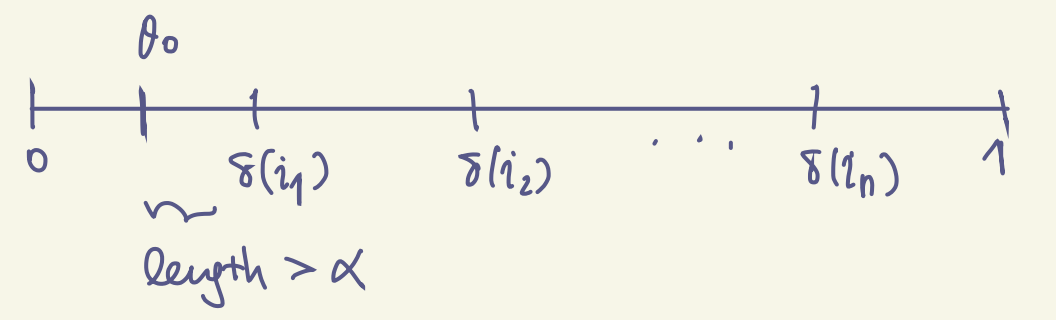
\includegraphics[width=0.7\textwidth]{figures/0-1loss.png}
    \caption{TO BE NAMED}
    \label{fig:01loss}
\end{figure}

\subsection{Admissibility of Minimax Estimator}

\begin{enumerate}
    \item Admissibility can give rise to minimaxity: 
    If $\delta$ is admissible with constant risk, 
    then $\delta$ is also minimax.
    \item Minimaxity does not guarantee admissibility: 
    It only ensures that the worst case risk is optimal\footnote{Recall Theorem \ref{thm:uniqbayesadm}, i.e. TPE 5.2.4.}.
\end{enumerate}

\begin{example}
    Let $X_1,\cdots,X_n\overset{iid}{\sim}\mathcal{N}(\theta,\sigma^2)$ with $\sigma^2$ known, 
    and $\theta$ is the estimated.
    Then the minimax estimator in $\Bar{X}_n$ under the squared error loss and we would like to 
    determine whether or not $\Bar{X}_n$ is admissible.

    \textbf{Question:} Let's try to answer a more general question: When is $a\Bar{X}_n+b$,
    for $a,b\in\mathbb{R}$ (i.e. affine function of $\Bar{X}_n$) admissible?
    \begin{enumerate}[{Case} 1]
        \item $0<a<1$:\\
        In this case $a\Bar{X}_n+b$ is a convex combination of $\Bar{X}_n$ and $b$.
        Bay our previous result,
        it is a Bayes estimator w.r.t. some Gaussian prior $\theta$.
        Since we adopt the squared error loss function,
        which is strictly convex,
        the Bayes estimator is unique.
        By Theorem \ref{thm:uniqbayesadm} (TPE 5.2.4, a unique Bayes estimator is always admissible),
        $a\Bar{X}_n+b$ is admissible.
        
        \item $a=0$:\\
        In this case $b$ is also a unique Bayes estimator w.r.t. 
        a degenerate prior distribution with the unique value at $\theta=b$,
        then by Theorem \ref{thm:uniqbayesadm}, b is also admissible.
        
        \item $a=1,b\neq{0}$:\\
        In this case $\Bar{X}_n+b$ is not admissible
        because it is dominated by $\Bar{X}_n$.
        Note that $\Bar{X}_n+b$ and $\Bar{X}_n$ have the same variance,
        but $\Bar{X}_n$ has a strictly smaller bias.
        
        \item $a>1$:\\
        In general, the risk of $a\Bar{X}_n+b$ is
        \begin{align}
            \mathbb{E}[a\Bar{X}_n+b-\theta]^2
            =& \mathbb{E}[a(\Bar{X}_n-\theta)+b+\theta(a-1)]^2\\
            =& \frac{a^2\sigma^2}{n} + [b+\theta(a-1)]^2\label{eq:caseadmiss}
        \end{align}
        In the case of $a>1$, by Equation \ref{eq:caseadmiss}, we have 
        \begin{gather}
            \mathbb{E}[a\Bar{X}_n+b-\theta]^2\geq\frac{a^2\sigma^2}{n}>\frac{\sigma^2}{n}=R(\theta,\Bar{X}_n)
        \end{gather}

        Hence, we conclude that $\Bar{X}_n$ dominates $a\Bar{X}_n+b$ 
        when $a>1$ in which case $a\Bar{X}_n+b$ is inadmissible.

        \item $a<0$:\\
        We have 
        \begin{align}
            \mathbb{E}[a\Bar{X}_n+b-\theta]^2
            >& [b-\theta(a-1)]^2\\
            =& (a-1)^2\left[\theta+\frac{b}{a-1}\right]^2\\
            >& \left[\theta-\left(-\frac{b}{a-1}\right)\right]^2
        \end{align}
        which is the risk of predicting with the constant $-\frac{b}{a-1}$.
        So, $-\frac{b}{a-1}$ dominates $a\Bar{X}_n+b$ and therefore $a\Bar{X}_n+b$ is again inadmissible.

        \item $a=1,b=0$:\\
        We shall proceed with a limiting Bayes argument.
        Suppose $\Bar{X}_n$ is inadmissible, then, WLOG,
        we let $\sigma^2=1$, we have $R(\theta,\Bar{X}_n)=\frac{1}{n}$.

        By our hypothesis, there must exist an estimator $\delta'$ such that
        $R(\theta,\delta')\leq\frac{1}{n}$ for all $\theta$ and 
        $R(\theta',\delta')<\frac{1}{n}$ for at least one $\theta'\in\Omega$.
        Because $R(\theta,\delta)$ is continuous in $\theta$, 
        there must exist $\varepsilon>0$ and an interval $(\theta_0,\theta_1)$ containing $\theta'$ such that
        \begin{gather}
            R(\theta,\delta')<\frac{1}{n}-\varepsilon~\forall{\theta}\in(\theta_0,\theta_1)\label{eq:caseadmiss2}
        \end{gather}

        Let $r'_\tau$ be the average risk of $\delta'$ w.r.t. the prior distribution $\mathcal{N}(0,\tau^2)$ on $\theta$.
        (We used the same prior to prove that $\Bar{X}_n$ was the limit of a Bayes estimator,
        and hence minimax.
        We did this by letting $\tau\to\infty$ (improper prior: $\pi(\theta)=1~\forall{\theta}$))
        Let $r_\tau$ be the average risk of a Bayes estimator $\delta_\tau$ under the same prior.
        Note that $\delta_\tau\neq\delta'$ because $R(\theta,\delta_\tau)\to\infty$ as $\theta\to\infty$,
        which is not consistent with $R(\theta,\delta')\leq\frac{1}{n}~\forall{\theta}\in\mathbb{R}$.
        So $r_\tau<r_\tau'$ because the Bayes estimator is unique almost surely w.r.t the marginal distribution of $\theta$.

        We shall look into the following ratio,
        which we shall show to become arbitrarily large and form a contradiction that $r_\tau<r_\tau'$.
        Using the form of the Bayes risk $r_\tau$, we can write
        \begin{gather}
            \frac{\frac{1}{n}-r_\tau'}
            {\frac{1}{n}-r_\tau}
            =
            \frac{\frac{1}{\sqrt{2\pi}\tau}
            \int_{-\infty}^\infty{
                \left[\frac{1}{n}-R(\theta,\delta')\right]\exp\left(-\frac{\theta^2}{2\tau^2}\right)
            }d\theta}
            {\frac{1}{n}-\frac{1}{n+1/\tau^2}}
        \end{gather}
        Applying Equation (\ref{eq:caseadmiss2}), we find:
        \begin{align}
            \frac{\frac{1}{n}-r_\tau'}{\frac{1}{n}-r_\tau}
            \geq& \frac{\frac{1}{\sqrt{2\pi}\tau}\int_{\theta_0}^{\theta_1}{
                \varepsilon\exp\left(-\frac{\theta^2}{2\tau^2}\right)
            }d\theta}
            {\frac{1}{n(n\tau^2+1)}}\\
            =& \frac{n(1+n\tau^2)\varepsilon}{\sqrt{2\pi}\tau}\int_{\theta_0}^{\theta_1}{
                \exp\left(-\frac{\theta^2}{2\tau^2}\right)
            }d\theta
        \end{align}
        As $\tau\to\infty$, the first expression $\frac{n(1+n\tau^2)\varepsilon}{\sqrt{2\pi}\tau}\to\infty$
        and since the integral converges monotonically to 1, 
        Lebesgue's MCT ensure that the integral approaches the positive quality $\theta_1-\theta_0$.
        So, for sufficiently large $\tau$, we must have 
        \begin{gather}
            \frac{\frac{1}{n}-r_\tau'}{\frac{1}{n}-r_\tau}
            > 1
            \iff 
            r_\tau'<r_\tau
        \end{gather}
        However this is a contradiction because $r_\tau$ is the optimal average risk
        since it is the Bayes risk.
        So our assumption that there was a dominating estimator $\delta$ is wrong
        and in this case $a\Bar{X}_n+b=\Bar{X}_n$ is admissible.
    \end{enumerate}
\end{example}

\subsection{Simultaneous Estimation}

So far, we consider only one parameter.

\begin{example}
    Let $X_1,\cdots,X_p$ be independent with $X_i\sim\mathcal{N}(\theta_i,\sigma^2)$
    for $1\leq{i}\leq{p}$.
    For the sake for simplicity, let $\sigma^2=1$.
    Our goal is to estimate $\boldsymbol{\theta}=(\theta_1,\cdots,\theta_p)^T$
    under the loss function 
    $L(\boldsymbol{\theta},\boldsymbol{d})=\sum_{i=1}^p(d_i-\theta_i)^2$.
    A natural estimator for $\boldsymbol{\theta}$ is $\boldsymbol{X}=(X_1,\cdots,X_p)^T$.
    It can be shown that $\boldsymbol{X}$ is the UMRUE,
    the MLE, a generalized Bayes and a minimax estimator for $\theta$.
    So it would be natural for us to think that $\boldsymbol{X}$ is admissible.
    However, it turns out that this is not the case when $p\geq{3}$.

    When $p\geq 3$, $\boldsymbol{X}$ is dominated by the James-Stein (J-S) estimator:
    \begin{gather}
        \delta(\boldsymbol{X})=(\delta_1(\boldsymbol{X}),\cdots,\delta_p(\boldsymbol{X}))
    \end{gather}
    where $\delta_i(\boldsymbol{X})=\left(1-\frac{p-2}{\|\boldsymbol{X}\|_2^2}\right)X_i$.
\end{example}
$~$\newline

Motivation for the J-S estimator (view it from the empirical Bayes framework):
\begin{enumerate}
    \item Suppose $\theta_i\overset{iid}{\sim}\mathcal{N}(0,A)$,
    then the Bayes estimator for $\theta_i$ is 
    \begin{gather}
        \delta_{A,i}(\boldsymbol{X})=\frac{X_i}{1+1/A}=\left(1-\frac{1}{A+1}\right)X_i
    \end{gather}
    \item We need to choose $A$:
    Marginalizing over $\theta$, we can show that $\boldsymbol{X}$ has the distribution
    \begin{gather}
        X_i\overset{iid}{\sim}\mathcal{N}(0,A+1)
    \end{gather}
    We may use $\boldsymbol{X}$ and the knowledge of this marginal distribution to find an estimate of $\frac{1}{A+1}$.
    Instead of using the M1E, we shall use an unbiased estimate.
    Considering that it can be shown that 
    \begin{gather}
        \mathbb{E}\frac{1}{\|\boldsymbol{X}\|_2^2}=\frac{1}{(p-2)(A+1)},~~~\left(\frac{\|\boldsymbol{X}\|_2^2}{A+1}\sim\chi^2_p\right)
    \end{gather}
    so $1-\frac{p-2}{\|\boldsymbol{X}\|_2^2}$ is UMVU for $1-\frac{1}{A+1}$.
\end{enumerate}

\begin{note}
    Note that
    \begin{align}
        \mathbb{E}\|\boldsymbol{X}\|_2^2
        =& \mathbb{E}\sum_{i=1}^pX_i^2
        = p + \sum_{i=1}^n{\theta_i^2}\\
        =& p + \|\boldsymbol{\theta}\|_2^2 > p.
    \end{align}
    $\Rightarrow$ We may view the J-S estimator as a method 
    for correcting the bias in the size of $\boldsymbol{X}$.\footnote{TPE 5.5.1 \& Keener 11.2}
\end{note}

\newpage